

%----------------------------------------------------------------------------------------
%	PACKAGES AND DOCUMENT CONFIGURATIONS
%----------------------------------------------------------------------------------------

\documentclass{article}
\usepackage[utf8]{inputenc}
\usepackage{appendix}
\usepackage[T1]{fontenc}
\usepackage[italian]{babel}
\usepackage{siunitx} % Provides the \SI{}{} and \si{} command for typesetting SI units
\usepackage{graphicx} % Required for the inclusion of images
\usepackage{natbib} % Required to change bibliography style to APA
\usepackage{amsmath} % Required for some math elements
\usepackage{caption}
\usepackage{tikz}


\usepackage{float}


\usetikzlibrary{arrows,automata, positioning}

\usepackage{import}

\setlength\parindent{0pt} % Removes all indentation from paragraphs

%----------------------------------------------------------------------------------------
%	DOCUMENT INFORMATION
%----------------------------------------------------------------------------------------

\title{Prova Finale di Reti Logiche} % Title
\author{Montanari Tommaso e Negri Riccardo} % Author name
\date{15 Maggio 2022}

\begin{document}
\maketitle % Insert the title, author and date
\begin{figure}[H]
	\centering
	
\includegraphics[width=0.365\textwidth]{Assets/logo.jpg}
\end{figure}
\begin{center}

\begin{tabular}{l l l l}
Docente: & Salice Fabio & & \\ 
Studente 1: & Montanari Tommaso & 10661941 & 932673\\
Studente 2: & Negri Riccardo & 10729927 & 936820 
\end{tabular}
\end{center}

\tableofcontents
\pagebreak

%----------------------------------------------------------------------------------------
%	SECTION 1
%----------------------------------------------------------------------------------------

\section{Introduzione}

La prova prevede l'implementazione in VHDL di un componente che opera su una memoria e svolge la seguente operazione: il componente deve per prima cosa leggere il primo byte dalla memoria che identifica il numero di parole che sono
state fornite come input, questa informazione è importante per capire quando la macchina deve terminare la lettura.

Dopodiché ogni parola successiva viene tradotta in due parole che vengono scritte progressivamente in un'altra parte della memoria a partire dall'indirizzo 1000.

Le parole di memoria sono interpretate dal codificatore come un flusso continuo e l'uscita è un flusso di lunghezza doppia. Visto che i byte vengono tradotti come un unico flusso l'output di una certa parola dipende anche da quelle precedenti e non possono essere processate separatamente.

\subsection{Codificatore Convoluzionale}
\begin{tikzpicture}[shorten >=1pt,node distance=3cm,node font=\small,on grid,auto,initial text={}]
	\tikzstyle{every state}=[fill={rgb:black,1;white,10}]
	
	\node[state,initial ]  (S01)                 {S01};
	\node[state]                    (S00) [below left of=S01]  {S00};
	\node[state]                    (S11) [below right of=S01]  {S11};
	\node[state]                    (S10) [below right of=S00]  {S10};
	
	\path[->]
	(S00) edge [loop left] node {0/00} ()
	(S11) edge [loop right] node {1/01} ()
	(S01) edge node [above, align=center] {0/11\\} (S00)
	(S00) edge node [below, align=center] {\\1/11} (S10)
	(S10) edge node [below, align=center] {\\1/10} (S11)
	(S11) edge node [above, align=center] {0/10\\} (S01)
	(S01) edge [bend left] node {1/00} (S10)
	(S10) edge [bend left] node {0/01} (S01);
\end{tikzpicture}

\subsection{Esempio}
Dato lo stato iniziale della memoria riportato di seguito il componente legge la prima parola che rappresenta la lunghezza dell'input (W=2). 
\\
\\
\begin{tabular}{c c c}
	Indirizzo & Valore & Codifica binaria \\
	0 & 2 & 0000 0010 \\
	1 & 35 & 0010 0011 \\
	2 & 161 & 1010 0001 \\
\end{tabular}
\\
\pagebreak
\\

Successivamente legge la parola presente all'indirizzo 1 e la elabora secondo il funzionamento del codificatore convoluzionale.  Essendo la prima parola letta il codificatore parte dallo stato S00. Di seguito sono riportati gli stream in input e output dal codificatore: 
\\
\\
\begin{tabular}{c c c}
	Stream & Codifica binaria & Parole corrispondenti \\
	Input &  0010 0011 & 35 \\
	Output & 0000 1101  1100 1110& 13 206 \\
\end{tabular}
\\
\\
\\
A seguito di questa codifica il codificatore convoluzionale si trova nello stato S11. Dopo avere scritto in memoria le due parole il componente legge la seconda, e ultima, parola ed esegue la codifica partendo con lo stato iniziale del codificatore pari a S11. Di seguito sono riportati gli stream in input e output dal codificatore: 
\\
\\
\begin{tabular}{c c c}
	Stream & Codifica binaria & Parole corrispondenti \\
	Input & 1010 0001 & 161 \\
	Output & 0110 0001 1100 0011 & 97 e 195 \\
\end{tabular}
\\
\\
\\
Le ulteriori due parole vengo quindi scritte in memoria e una volta concluso il processo la memoria appare come rappresentato di seguito.
\\
\\
\begin{tabular}{c c c}
	Indirizzo & Valore & Codifica binaria \\
	1000 & 13 & 0000 1101 \\
	1001 & 206 & 1100 1110 \\
	1002 & 97 & 0110 0001 \\
	1003 & 195 & 1100 0011 \\
\end{tabular}
\\
\\

\subsection{Ipotesi Progettuali}
\begin{itemize}
\item {Per lo sviluppo del componente si è utilizzata una scheda Artix-7 FPGA xc7a200tfbg484-1.}
\item {Ogni byte può contenere numeri da 0 a 255.}
\item {La quantità di numeri in ingresso (W) è contenuta in una parola da un byte quindi anche il numero massimo di parole da tradurre è 255.}
\item {Dato che l'input occupa al massimo 256 byte è possibile scrivere in memoria a partire dai byte successivi. Da specifiche si scrive sempre a partire dall'indirizzo 1000 che quindi sicuramente non conterrà l'input.}
\end{itemize}



%----------------------------------------------------------------------------------------
%	SECTION 2
%----------------------------------------------------------------------------------------

\section{Architettura}
L'implementazione è stata realizzata in un solo modulo per semplicità, si possono distinguere due parti all'interno della macchina che cooperano per raggiungere il risultato. È presente una macchina che simula il funzionamento dell'automa a stati finiti fornito nella specifica che rappresenta il codificatore convoluzionale, è responsabile della traduzione uno a due dei bit. Inoltre è presente una seconda macchina principale che si occupa della lettura e scrittura dei flussi di bit e tratta la prima come una scatola nera. Ciascuna macchina ha un segnale distinto che contiene il suo stato.

\subsection{Interfaccia}
\begin{itemize}
	\item \textbf{i\_clk:} Segnale di clock
	\item \textbf{i\_rst:} Segnale di reset, deve riportare la macchina allo stato iniziale.
	\item \textbf{i\_start:} Quando viene portato a 1 la macchina comincia ad operare e prima di terminare aspetta che sia riportato a 0 (handshake).
	\item \textbf{i\_data:} Vettore da 8 bit che contiene il la parola di memoria che è stata letta.
\end{itemize}

\begin{itemize}
	\item \textbf{o\_address:} Un vettore di 16 bit che contiene l'indirizzo della parola da scrivere o da leggere.
	\item \textbf{o\_done:} Quando la macchina ha finito l'esecuzione viene portato a 1 e aspetta che i\_start sia 0 poi anche 0\_done è riportato a 0 (handshake).
	\item \textbf{o\_en:} Se settato a 1 richiede l'operazione di lettura o scrittura.
	\item \textbf{o\_we:} Se settato a 1 l'operazione richiesta da o\_en è scrittura altrimenti è lettura.
	\item \textbf{o\_data:} Vettore da 8 bit che contiene il la parola di memoria da scrivere.
\end{itemize}
\pagebreak
\subsection{Descrizione ad alto livello}
Questa è la descrizione a parole delle fasi che l'esecuzione segue. All'interno del componente ciascuna di queste diverse fasi corrisponde ad uno stato (o a più stati).

\begin{enumerate}
	\item Inizio:
	\begin{enumerate}
		\item Legge il primo byte di memoria contenente la lunghezza dell'input e salva il valore in un segnale.
		\item Inizializza l'indirizzo di lettura al secondo byte e quello di scrittura al byte 1000.
	\end{enumerate}
	\item Traduzione:
	\begin{enumerate}
		\item Legge un byte e sposta il punto di lettura.
		\item Simula un passo dell'automa del codificatore usando in ingresso un bit dal byte appena letto e aggiungendo due bit al segnale di output. (Ripetuto 4 volte)
		\item L'output dell'automa ora contiene 8 bit quindi viene salvato in una parola di memoria e si incrementa l'indirizzo di scrittura.
		\item Se sono rimasti bit da tradurre nel byte letto torna al punto 2.b
		\item Altrimenti se sono rimasti byte da leggere torna al punto 2.a
		\item Altrimenti termina.
	\end{enumerate}
\end{enumerate}

Ogni operazione di lettura nella memoria si scompone in più stati nel programma: richiesta della lettura, attesa della fine dell'operazione, utilizzo del dato letto o salvataggio in un segnale. 

\subsection{Diagramma degli stati}


% { \epsilon }
\begin{tikzpicture}[shorten >=1pt,node distance=3cm,node font=\small,on grid,auto,initial text={begin}]
	\tikzstyle{every state}=[fill={rgb:black,1;white,10}]
	
	\node[state,text width=1.5cm,align=center,initial ]  (START)                 {START};
	\node[state,text width=1.5cm,align=center]                    (WWN) [right of=START]  {WAIT\\WORDS\\NUMBER};
	\node[state,text width=1.5cm,align=center]                    (FWN) [right of=WWN]  {FETCH\\WORDS\\NUMBER};
	\node[state,text width=1.5cm,align=center]                    (DONE) [below of=WWN]  {DONE};
	\node[state,text width=1.5cm,align=center]                    (AD) [left of=DONE]  {AFTER\\DONE};
	\node[state,text width=1.5cm,align=center]                    (CR) [below right of=FWN]  {CALL\\READ};
	\node[state,text width=1.5cm,align=center]                    (WR) [below right  of=CR]  {WAIT\\READ};
	\node[state,text width=1.5cm,align=center]                    (FR) [below of=WR]  {FETCH\\READ};
	\node[state,text width=1.5cm,align=center]                    (WRITE) [below of=DONE]  {WRITE};
	\node[state,text width=1.5cm,align=center]                    (E12) [below left of=FR]  {ENCODER\\1 TO 2};
	
	\path[->]
	(START) edge [bend left] node [above] {i\_start = '1'} (WWN)
	(WWN) edge (FWN)
	(FWN) edge [bend left] node {i\_data = 0} (DONE)
	(FWN) edge [bend left] node {i\_data $\ne$ 0} (CR)
	(CR) edge [bend left] (WR)
	(WR) edge (FR)
	(FR) edge [bend left](E12)
	(E12) edge [loop below] node [align=center] {w\_word\_index ha\\qualsiasi altro valore} ()
	(E12) edge [bend right] node [above,align=right] {\\\\w\_word\_index\\= 0 or 4} (WRITE)
	(WRITE) edge [bend right] node [below,align=center] {\\not\\finished\_reading} (E12)
	(WRITE) edge node {words\_left = 0} (DONE)
	(WRITE) edge [bend right] node [align=center] {finished\_reading} (CR)
	(DONE) edge (AD)
	(AD) edge node {i\_start = '0'} (START);
\end{tikzpicture}
\\
\\
\begin{itemize}
	\item \textbf{START:} Lo stato in cui la macchina è all'inizio dell'esecuzione del programma. In presenza del segnale i\_state = '1' imposta valori iniziali, fa la richiesta di lettura all'indirizzo 0 e passa allo stato successivo.
	\item \textbf{WAIT\_WORDS\_NUMBER:} Un ciclo di clock dopo che la lettura è stata richiesta riporta a 0 il segnale o\_en.
	\item \textbf{FETCH\_WORD\_NUMBER:} Dopo la fine della lettura salva il numero di byte in input nel segnale words\_left. Nel caso particolare in cui ci sono 0 byte in ingresso passa direttamente allo stato DONE, altrimenti incomincia con la lettura del primo byte.
	\item \textbf{CALL\_READ:} Richiede la lettura e imposta l'indirizzo corretto.
	\item \textbf{WAIT\_READ:} Un ciclo di clock dopo che la lettura è stata richiesta porta a 0 il segnale o\_en.
	\item \textbf{FETCH\_READ:} Dopo che la lettura è terminata salva il valore letto in w\_word.
	\item \textbf{ENCODER\_1\_TO\_2:} In questo stato viene simulato il codificatore che effettua la traduzione, lo stato di tale automa è salvato in un segnale separato chiamato internal\_state. Ogni 4 bit tradotti z\_word, ovvero la parola da un byte in uscita, è piena e quindi si passa alla scrittura di tale parola in memoria.
	\item \textbf{WRITE:} Scrive z\_word in memoria. Dopodiché se rimangono dei bit da leggere in w\_word torna allo stato dell'encoder. Se la parola è finita ma ci sono altre parole in input da leggere torna a CALL READER, se tutte le parole sono state tradotte allora passa a DONE.
	\item \textbf{DONE:} Porta il segnale o\_done a 1.
	\item \textbf{AFTER\_DONE:} Prima di tornare allo stato START si assicura che il segnale i\_start che era stato dato all'inizio sia stato riportato a 0 e in tal caso riporta a 0 il segnale o\_done.
\end{itemize}
\pagebreak
%----------------------------------------------------------------------------------------
%	SECTION 3
%----------------------------------------------------------------------------------------

\section{Risultati sperimentali}
\subsection{Sintesi}
Il componente sviluppato è sintetizzabile ed implementabile. 
\begin{figure}[H]
	\centering
	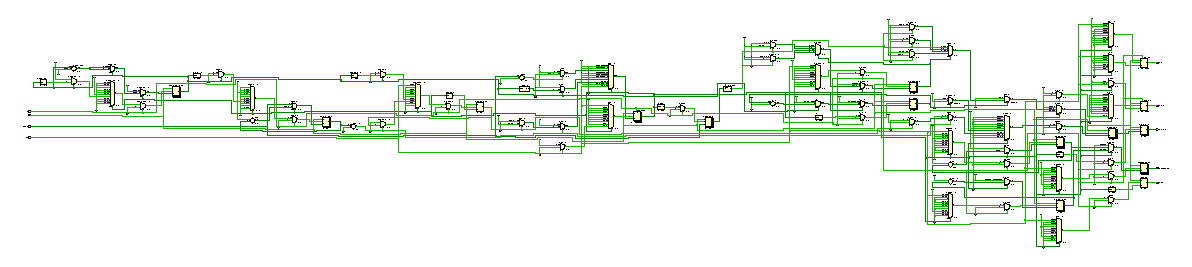
\includegraphics[width=1\textwidth]{Assets/schematic.eps}
	\caption{Schema post-sintesi}
\end{figure}
Nella seguente tabella sono indicati i componenti utilizzati nella sintesi.
\begin{center}
	\begin{tabular}{c|c|c|c}
		
		Site Type   & Used & Available & Utilization\% \\
		\hline
		LUT as Logic & 117 & 134600 & 0.09 \\
		
		Register as Flip Flop & 95 & 269200  & 0.04\\
		
		F7 Muxes & 1 & 67300 & <0.01\\
		
	\end{tabular}
\end{center}



\subsection{Simulazioni}
Al fine di verificare il corretto funzionamento del componente sono stati eseguiti diversi test bench in simulazioni Behavioural, Post-synthesis functional e Post-synthesis timing. 
Di seguito sono riportati i test significativi effettuati con relativa spiegazione, tempi ottenuti e grafico d'onda.

\subsubsection{Flussi successivi}
Tramite questo test si verifica la correttezza  nel caso di codifica di più flussi uno dopo l'altro. Nel testbench usato vengono codificati tre flussi (senza reset dopo ogni flusso).
\begin{description}
	\item[Behavioural] 21850 ns
	\item[Post-synthesis functional] 22350100 ps
	\item[Post-synthesis timing] 22353714 ps
\end{description}
\begin{figure}[H]
	\centering
	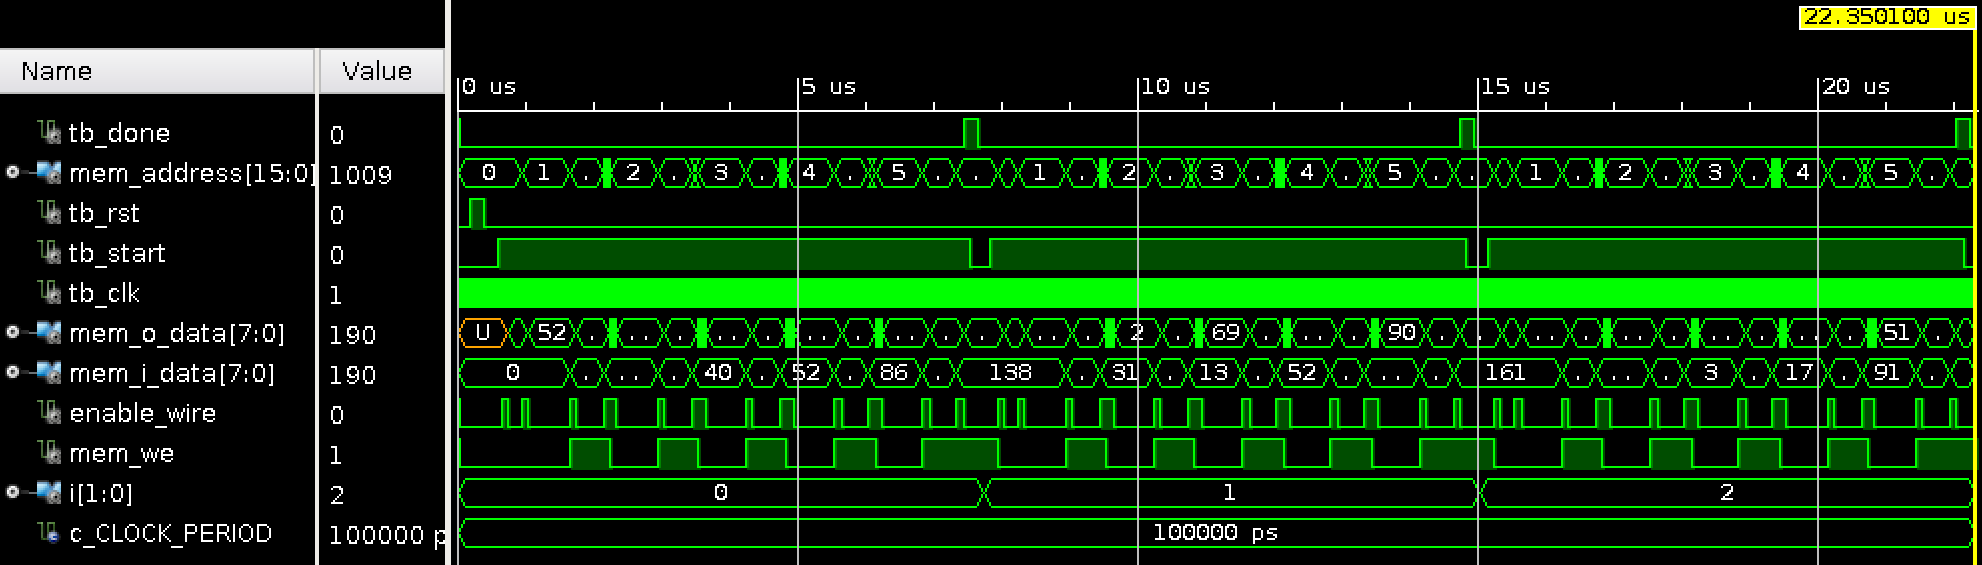
\includegraphics[width=1\textwidth]{Assets/tb1.png}
	\caption{Post-synthesis functional simulation waveform}
\end{figure}

\subsubsection{Reset asincrono}
Tramite questo test si verifica il corretto funzionamento del reset asincrono.
\begin{description}
	\item[Behavioural] 10650 ns
	\item[Post-synthesis functional] 10750100 ps
	\item[Post-synthesis timing] 10753714 ps
\end{description}
\begin{figure}[!htb]
	\centering
	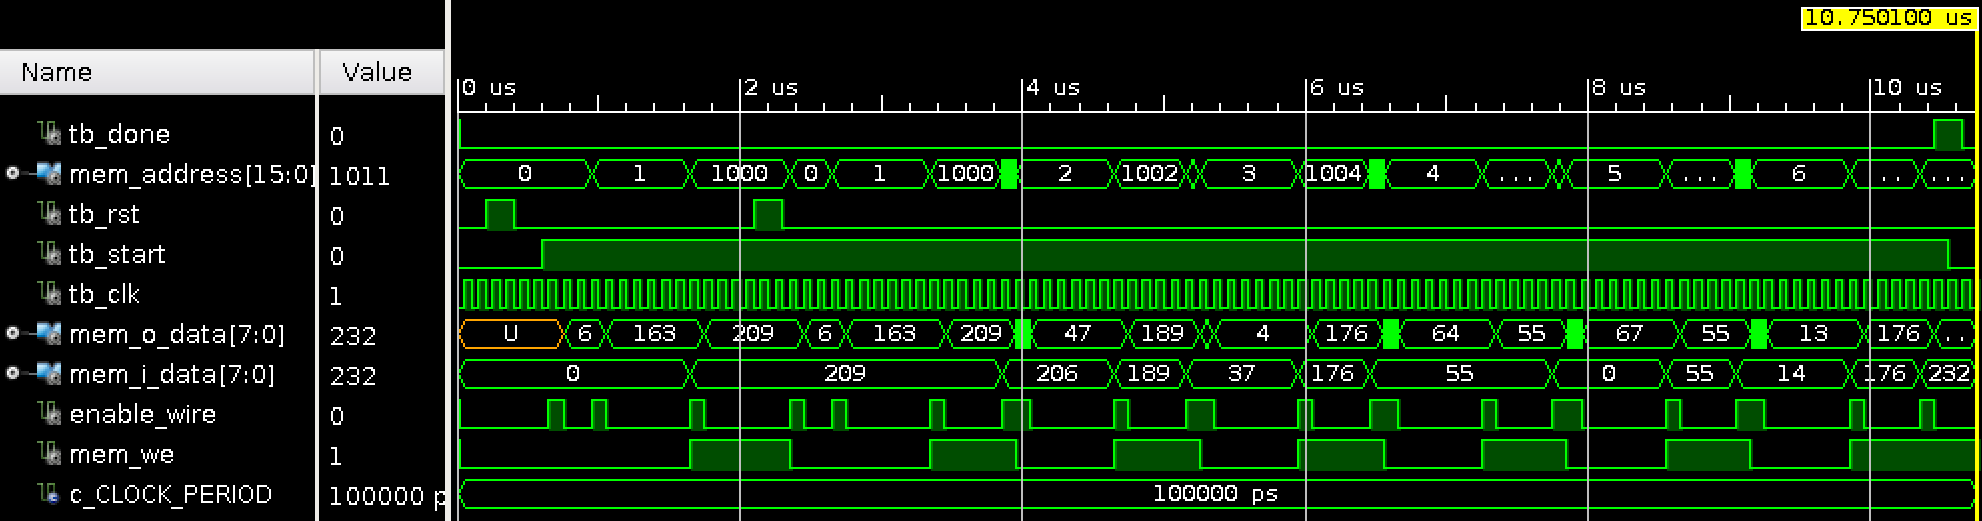
\includegraphics[width=1\textwidth]{Assets/tb2.png}
	\caption{Post-synthesis functional simulation waveform}
\end{figure}

\subsubsection{Sequenza di lunghezza massima}
\paragraph{}Tramite questo test si verifica il corretto funzionamento nel caso di sequenza di ingresso di lunghezza massima: 255 byte.
\begin{description}
	\item[Behavioural] 332450 ns
	\item[Post-synthesis functional] 332550100 ps
	\item[Post-synthesis timing] 332553714 ps
\end{description}
In questo caso non si riporta grafico della forma d'onda perché non è possibile distinguere i valori che i segnali assumono nella vista "fit".
%\begin{figure}[!htb]
%	\centering
%	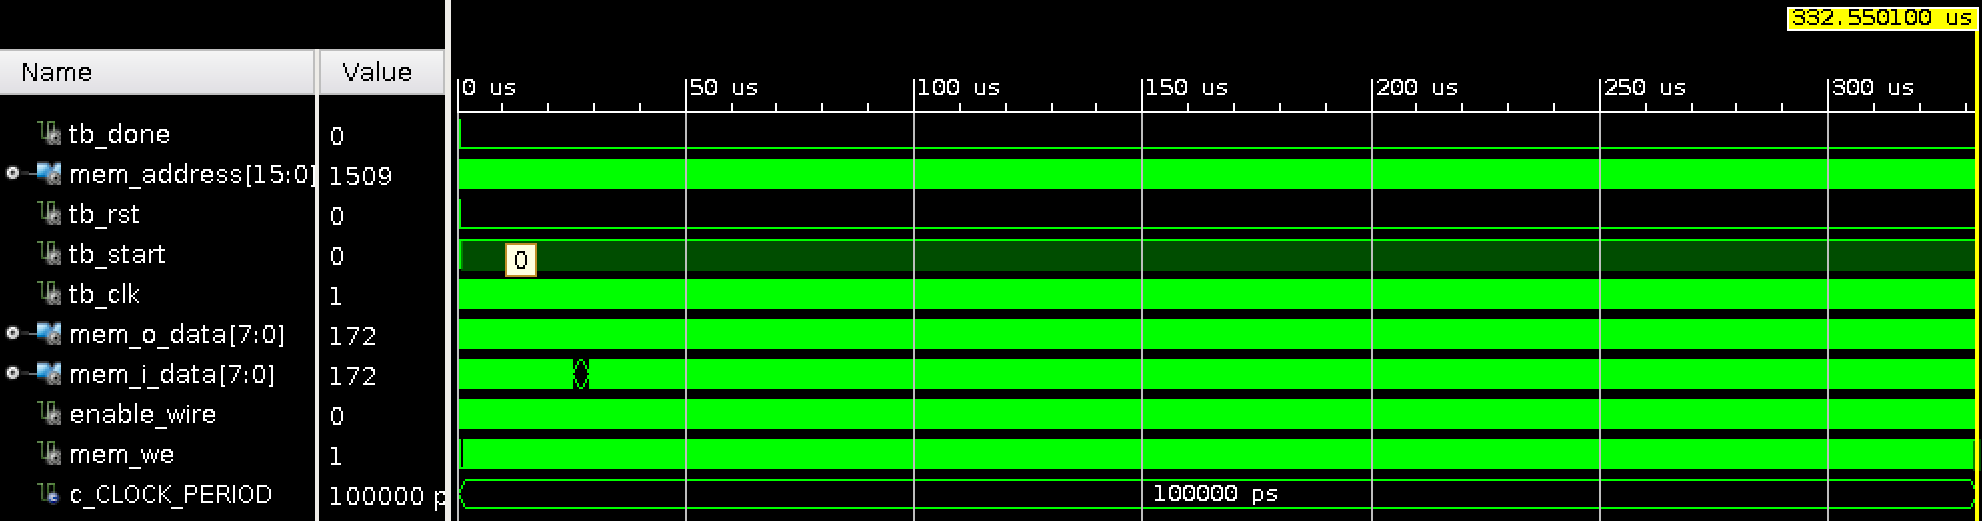
\includegraphics[width=1\textwidth]{Assets/tb3.png}
%	\caption{Post-synthesis functional simulation waveform}
%\end{figure}

\subsubsection{Sequenza di lunghezza nulla}
Tramite questo test si verifica il corretto funzionamento nel caso di sequenza di ingresso di lunghezza minima: 0 byte.
\begin{description}
	\item[Behavioural] 950 ns
	\item[Post-synthesis functional] 1050100 ps
	\item[Post-synthesis timing] 1053714 ps
\end{description}
\begin{figure}[H]
	\centering
	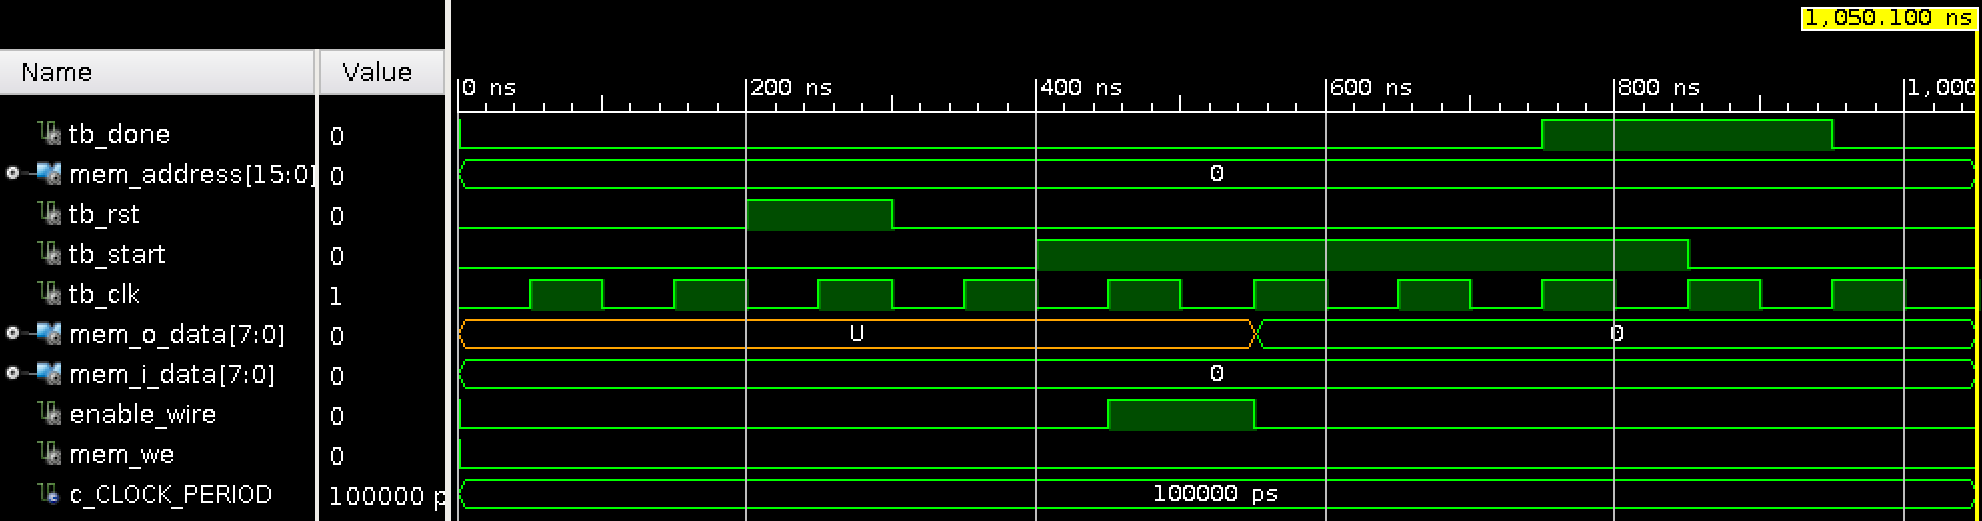
\includegraphics[width=1\textwidth]{Assets/tb4.png}
	\caption{Post-synthesis functional simulation waveform}
\end{figure}

\subsubsection{Tests con reset}
Test bench, con reset dopo ogni test, che effettua 1000 test (generati casualmente con uno script Python) per testare ulteriormente il componente.
\begin{description}
	\item[Behavioural] 172743250 ns
	\item[Post-synthesis functional] 172943150100 ps
	\item[Post-synthesis timing] 172943153714 ps
\end{description}
In questo caso non si riporta grafico della forma d'onda perché non è possibile distinguere i valori che i segnali assumono nella vista "fit".

\subsubsection{Tests senza reset}
Test bench, senza reset dopo ogni test, che effettua 1000 test (generati casualmente con uno script Python) per testare ulteriormente il componente.
\begin{description}
	\item[Behavioural] 172543450 ns
	\item[Post-synthesis functional] 172743350100 ps
	\item[Post-synthesis timing] 172743353714 ps
\end{description}
In questo caso non si riporta grafico della forma d'onda perché non è possibile distinguere i valori che i segnali assumono nella vista "fit".
\pagebreak
%----------------------------------------------------------------------------------------
%	SECTION 4
%----------------------------------------------------------------------------------------

\section{Conclusioni}
A seguito di estensivo testing effettuato tramite test bench scritti sia manualmente che generati casualmente, si ritiene che l’architettura progettata rispetti le specifiche. Reputiamo inoltre il componente adeguatamente robusto perché ha soddisfatto le specifiche anche in casi limite.
\\
\\
Nella realizzazione del componente in VHDL si è utilizzato un singolo process per avere una maggiore chiarezza, un minore utilizzo di segnali e avere un codice molto leggibile.
\\
\\
Il design è risultato sintetizzabile ed implementabile. La soluzione adottata sfrutta quasi interamente LUT e Flip Flop fatta eccezione per un F7 Muxes, non fa quindi uso di Latch.
\\

%----------------------------------------------------------------------------------------

\end{document}